\chapter{Projektformulering} \label{ch:projektformulering}
\section{Problemformulering} \label{sec:problemformulering}
Ifølge Niklas Alexander Chimirri, forsker inden for områder som barndom, psykologi og teknologi ved Roskilde Universitet, er leg en vigtig del af børns opvækst.   
Det er essentielt for deres fremtid da det gør børnene sociale, robuste, kreative og ikke mindst nysgerrige. Med til at skabe rammerne for børns leg er legetøj, og i dag er det vigtigt at børn har mulighed for at anvende den teknologi der er til rådighed i dagens Danmark. 
Dette bekræftes i en artikel der er udgivet på Roskilde Universitets hjemmeside i november 2014.
Han konkluderer at der er for stor forskel imellem den virkelighed børnene møder i, og uden for børnehaven ift. den teknologi der i dag er til rådighed. 

%TODO Indsæt kildehenvisning: https://www.ruc.dk/om-universitetet/nyhedsportal/rubrik-forskningsmagasin/rubrik-nr-6/voksne-skal-forstaa-boerns-leg-med-teknik/

%---------------------------------------------------------------------------------------
%											PROJEKTBESKRIVELSE
%---------------------------------------------------------------------------------------

\section{Projektbeskrivelse} \label{sec:beskrivelse}


Projektet skal bidrage til eller i det mindste sætte fokus på, at det er vigtigt at børn har muligheden for at lege... og gerne med moderne teknologi. Derfor omhandler projektet design og implementering af en fjernstyret bil. Det skal ikke være en almindelig fjernstyret bil - den skal være intelligent og den får navnet ’’AU2’’. En skitse af bilen er vist på figur \ref{fig:rigbillede}.

Den intelligente del består af sensorer samt en kommunikationsenheder, som gør det muligt at styre bilen over et trådløst netværk. Brugeren har hermed mulighed for at navigere bilen ved at betragte en computerskærm, der viser et live-stream med video fra et kamera monteret på bilen. Er bilen inden for synsfeltet kan den selvfølgelig også styres ved at se direkte på den. For at undvige forhindringer på kørebanen, implementeres et anti-kollisionssystem bestående af afstandssensorer på bilen, placeret sådan at de kan detektere om bilen nærmer sig en forhindring. Således kan bilen selv kan standse eller undvige, hvis den nærmer sig en forhindring hastigt. Anti-kollisionssystemet har til formål at  forhindre en evt. kollision og derved beskadigelse af bilen eller dens omgivelser.

\begin{figure}[h]
\centering
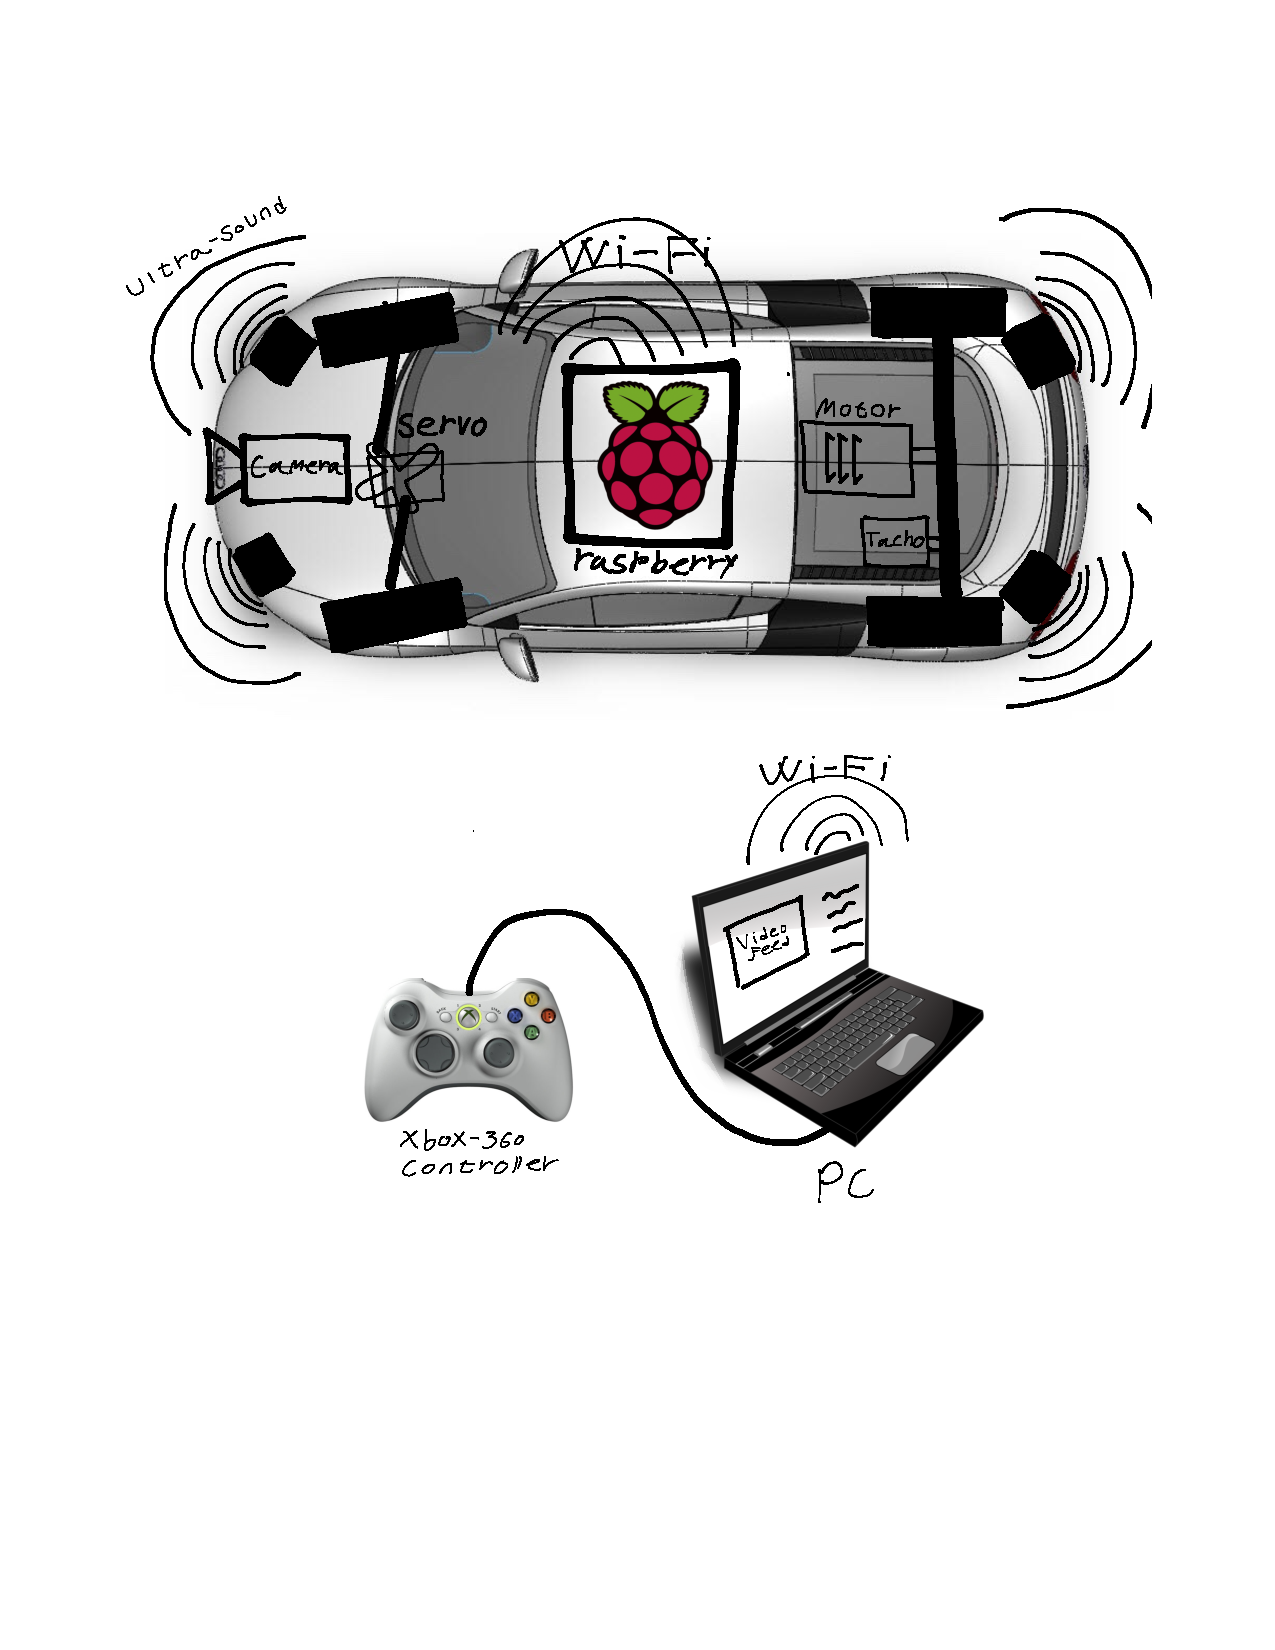
\includegraphics[width=\textwidth - 7.38 cm]{../fig/billeder/rigbillede}
\caption{Rigt billede af systemet i sin helhed}
\label{fig:rigbillede}
\end{figure}